\section{Foundational Agentic Reasoning}
\label{sec:foundational}

Agentic reasoning originates from the behavior of a single agent. 
Before discussing adaptation and collaboration, we focus on how an individual agent translates reasoning into structured action through three core components: \emph{planning}, \emph{search}, and \emph{tool use}. 
In this setting, the agent is not a passive text generator but an autonomous problem solver that formulates plans, explores alternatives through retrieval or environment search, and leverages tools to execute grounded operations. 
Together, these mechanisms establish the foundation of agentic reasoning, linking abstract deliberation with verifiable action.

A canonical foundational workflow can be viewed as an iterative cycle that interleaves 
\textbf{planning} (goal decomposition and task formulation),  \textbf{tool use} (invoking external systems or APIs to act on the world) and \textbf{search} (retrieval and exploration for decision support), 
Reasoning serves as the organizing principle across these stages, determining when to plan, what to retrieve, and how to act, transforming static inference into interactive decision-making.

By analyzing these components, we clarify how structured reasoning elevates a static LLM into an autonomous, goal-driven agent. 
The next section introduces \textbf{self-evolving reasoning}, where \emph{feedback} and \emph{memory} enable continual adaptation and extension of these foundational capabilities. 
Subsequently, we examine \textbf{collective reasoning}, in which multiple agents coordinate through roles, communication, and shared memory to achieve objectives beyond individuals.



\subsection{Planning Reasoning} % (ToT, ReWOO, hierarchical)


Planning is a central component of intelligent behavior, enabling agents to decompose problems, sequence decisions, and navigate complex environments with foresight. Recent research has increasingly explored planning in the context of large language models (LLMs), either as autonomous agents or as components in broader systems. In this section, we categorize existing work in agent planning for reasoning into six methodological styles, where each category highlights a distinct planning strategy that supports complex agentic reasoning. 

\begin{figure}
    \centering
    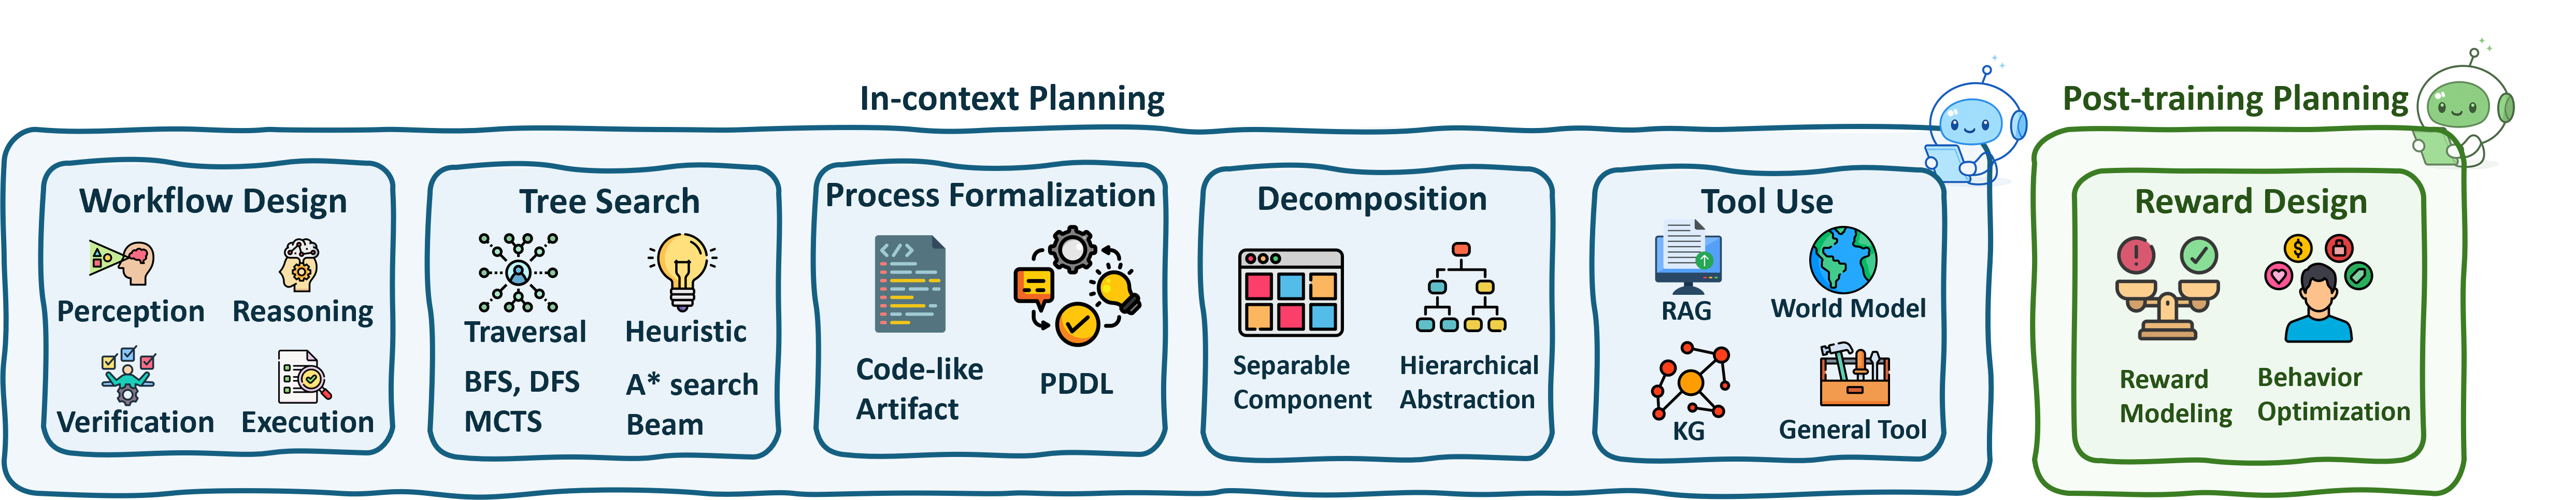
\includegraphics[width=\linewidth]{arxiv/figs/planning.png}
    \caption{Overview of \textbf{Planning Reasoning} in LLM agents, categorized into in-context planning and post-training planning.}
    \label{fig:planning}
\end{figure}

\begin{table*}[!t]
% \newcommand\TODO{\textcolor{magenta}{[TODO]}}
\centering
\caption{Representative \textbf{Agentic Planning} systems categorized by \textit{Modality}, \textit{Structure}, \textit{Format}, and \textit{Tool}.}
\renewcommand{\arraystretch}{1.15}
\setlength{\tabcolsep}{6pt}
\begin{tabular}{p{3cm}>{\centering\arraybackslash}p{3cm}>{\centering\arraybackslash}p{4cm}>{\centering\arraybackslash}p{5.5cm}}
\toprule
\textbf{Method} & \textbf{Structure} & \textbf{Format} & \textbf{Tool} \\
\midrule
\rowcolor[HTML]{F5F5F5}
\multicolumn{4}{l}{\textbf{Modality I: Language Agents (e.g., Search Agents, Code Agents)}} \\
ReWOO~\cite{xu2023rewoo} & Decomposed & Natural Language & None \\
Reflexion~\cite{shinn2023reflexion} & Sequential & Natural Language & None \\
LLM+P~\cite{liu2023llmp} & Sequential & Formal Language & None \\
IPC~\cite{valmeekam2023planning} & Sequential & Formal Language & None \\
ToT~\cite{yao2023tree} & Tree & Natural Language & None \\
GoT~\cite{besta2024graph} & Graph & Natural Language & None \\
AoT~\cite{sel2023algorithm} & Graph & Natural Language & None \\
HTP~\cite{gui2025hypertree} & Hypertree & Natural Language & Retrieval \\
RefPlan~\cite{jeong2025reflect} & Tree & Constrained Space & None \\
Gorilla~\cite{patil2024gorilla} & Sequential & Programming Language & Retrieval, API \\
CodeNav~\cite{gupta2024codenav} & Sequential & Programming Language & Code Indexer, Code Search \\
PoG~\cite{chen2024plan} & Graph & Natural Language & Knowledge Graph \\
Tool-Planner~\cite{liu2025toolplanner} & Sequential & Natural Language & Tool Cluster \\
\midrule
\rowcolor[HTML]{F5F5F5}
\multicolumn{4}{l}{\textbf{Modality II: Visual/Multimodal Agents (e.g., GUI Agents, Embodied Agents)}} \\
VisualPredictor~\cite{liang2024visualpredicator} & Tree & Formal Language & None \\
LLM-Planner~\cite{song2023llmplannerfewshotgroundedplanning} & Sequential & Formal Language & Object Detector, KNN \\
Agent-E~\cite{abuelsaad2024agent} & Sequential & Formal Language & DOM Grounder, Screenshot \\
Agent S~\cite{agashe2024agent} & Hierarchical & Natural Language & API, Search, Memory \\
ExRAP~\cite{yoo2024exploratory} & Sequential & Natural Language & Memory \\
AESOP~\cite{sinha2024real} & Reactive & Natural Language & Anomaly Detector \\
HRV~\cite{cornelio2025hierarchical} & Hierarchical & Formal Language & Symbolic Verifier \\
BehaviorGPT~\cite{zhou2024behaviorgpt} & Sequential & Visual Features & World Model \\
Dino-WM~\cite{zhou2024dino} & Tree & Visual Features & World Model \\
FLIP~\cite{gao2024flip} & Sequential & Visual Features & Language Model \\
\bottomrule
\end{tabular}
\label{tab:agentic_planning_methods}
\end{table*}

\subsubsection{In-context Planning}
\paragraph{Workflow Design.} Workflow-based approaches often emphasize structuring the overall planning process into distinct stages (e.g., perception, reasoning, execution, verification), which are either explicitly scaffolded or learned implicitly. For example, \cite{liu2023llmp,valmeekam2023planning,xu2023rewoo,hao2024llm} design planning pipelines that decompose task solving into subtasks, often leveraging a deliberate plan-and-act framework. Similarly, \cite{zhou2022least,wang2023plan,sel2023algorithm,shen2023hugginggpt} rely on structured prompting to sequentialize tasks and guide reasoning progression. Methods like \cite{liu2023plan} use structured transitions between diverse ``X-of-Thought'' strategies. PERIA \cite{ni2024peria} combines perception, imagination, and action in a unified multimodal workflow. Others such as \cite{erdogan2025plan} explicitly target long-horizon planning through structured sequencing, while \cite{wen2024codeplan} build workflows for code-related planning. 


These workflows are then grounded by a reactive controller that iteratively consumes the current state and interleaves reasoning with actions: in web automation, agents follow inspect-reason-act-observe loops \cite{yao2023react,deng2023mind2web}, with robustness improved by dynamically adapting in-context examples \cite{lutz2024wilbur}; in code, agents decide immediate executions/API calls, read outputs or errors, and refine step-by-step \cite{wang2024executable,patil2024gorilla,shinn2023reflexion,gupta2024codenav,rahman2025marco,he2024enhancing,rawat2025pre,aksitov2023rest,jiang2024self}; in robotics, monitors trigger on-the-fly safety interventions and VLM-guided subgoal execution with real-time adjustment \cite{sinha2024real,shah2023lm}. This \emph{reactive workflow} view unifies scripted stage design with online adaptation: the workflow provides interpretable structure and interfaces (what is done when), while the reactive loop supplies closed-loop grounding and error recovery (how it is done in context). The approach is broadly effective yet can accumulate errors over long horizons, motivating incremental verification and memory within the workflow to stabilize execution.


\paragraph{Tree Search / Algorithm Simulation.} Tree-based search strategies, especially BFS, DFS, A*, MCTS, and beam search, have become prominent as interpretable and effective planning scaffolds. Several works simulate tree traversal algorithms to mimic deliberative processes: \cite{yao2023tree,markowitz2024tree,long2023large,koh2024tree} apply breadth- or depth-first strategies to explore structured thought trees. A*-like guided expansions appear in \cite{wang2024qstar,meng2024llmastar,liu2024multimodal}, providing heuristic-driven planning with state evaluation. Besides that, MCTS is heavily explored in agentic research: \cite{hao2023reasoning,putta2024agent,sprueill2023monte,yu2023prompt,zhao2023large,ding2023everything,chen2024tree,kong2024latent,feng2023alphazero,yoon2025monte,schultz2024mastering,chen2025broaden} use MCTS or its variations for controlled exploration and improved reasoning fidelity. Beam search is leveraged in \cite{xie2023self,golovneva2023pathfinder,qian2025discriminator} to prune and prioritize reasoning trajectories efficiently. Other tree-search-inspired works include \cite{gandhi2024stream} which uses learned search policies and \cite{saha2024system} which differentiates between fast (reactive) and slow (deliberative) planning. These methods mirror traditional algorithmic planning, grounding LLMs' search processes in classical decision-making frameworks.

This search-over-hierarchy view maps cleanly onto domain systems. In the web setting, planner-executor architectures generate high-level subtask trees in natural language and bind leaves to DOM-grounded actions, often with memory to persist context \cite{abuelsaad2024agent,guan2023intelligent,agashe2024agent}. For code agents, hierarchical task trees and pseudo-code plans recursively break problems into compilable/editable units, while structured pipelines embed hierarchical RL or MCTS within the tree to choose promising edits and verification paths \cite{gui2025hypertree,ni2024tree,chen2025enhancing,hu2025divide,antoniades2024swe}. In robotics, behavior trees and high-level goal decomposition translate language instructions into subgoal sequences executed by low-level controllers and skills \cite{lykov2024llm,cao2023robot,izzo2024btgenbot,ahn2022icanisay,huang2022inner}. 

Taken together, hierarchical tree-search couples \emph{plan synthesis} (node expansion, heuristic/evidence-based selection) with \emph{plan realization} (leaf grounding and feedback), yielding interpretable, long-horizon agents that can backtrack, refine, and verify before committing to irreversible actions, while remaining flexible enough to incorporate learned policies and memory for efficiency and robustness.


\paragraph{Process Formalization.} Formalizing planning through symbolic representations, programming languages, or logic frameworks ensures compositionality, interpretability, and generalization. Several works encode plans as code-like artifacts or PDDL programs: \cite{guan2023leveraging,mahdavi2024leveraging,katz2024thought,wen2024codeplan,hao2024planning,vyas2024llm} incorporate symbolic logic or procedural programming into LLM prompting or output generation. These representations enable downstream tool execution and interface more cleanly with classical planners or robot controllers. PDDL-based formulations explicitly bridge LLM planning with well-established planning ecosystems, as in \cite{mahdavi2024leveraging,katz2024thought}. CodePlan \cite{wen2024codeplan} highlights the use of program synthesis to scaffold long-horizon reasoning. Such formalization provides structural scaffolds for agent behavior and often enhances explainability and robustness of the generated plans.

\paragraph{Decoupling / Decomposition.} Decoupling strategies aim to modularize complex planning into separable components such as goal recognition, memory retrieval, and plan refinement. Notably, ReWOO \cite{xu2023rewoo} explicitly separates observation and reasoning modules to optimize for efficiency. Similarly, works like \cite{zhang2025atomic, dong2024diffuserlite,lo2024goal,li2024agent,wang2023goplan,vyas2024llm,kang2025retrointext} break reasoning into reusable or hierarchical abstractions. \cite{gui2025hypertree} promotes hierarchical thinking through hypertrees, while \cite{liang2024visualpredicator} abstracts the world with symbolic predicates to reduce planning burden. Others, such as \cite{ye2024beyond} and \cite{kong2024latent}, decompose via latent variables or state spaces. These decompositions not only enhance tractability, but also align with neural-symbolic hybrid frameworks. They are especially common in long-horizon or multi-agent planning scenarios, such as \cite{zheng2024planagent,nayak2024long}.\nocite{wei2024robust,bao2025latte,chen2024wapiti,liu2025breaking,liu2024logic,liu2024class,liu2024aim,liu2023topological,zeng2025pave,zeng2024graph,lin2025moralise,lin2024backtime,qiu2025saffron,qiu2025ask,qiu2025efficient,qiu2024tucket,qiu2023reconstructing,qiu2022dimes,xu2024discrete,li2025model,zou2025transformer,qiu2024gradient,yoo2025embracing,yoo2025generalizable,yoo2024ensuring,chan2024group,wu2024fair,he2024sensitivity,wang2023networked}

\paragraph{External Aid / Tool Use.} Many systems leverage external structures or tools to aid planning, including retrieval-augmented generation (RAG), knowledge graphs, world models, and general-purpose tool use. Knowledge-augmented frameworks like \cite{chen2024plan,cornelio2025hierarchical,meng2025telograf,zhong2024flexplanner, zhang2025atomic} inject structured representations (e.g., graphs, scene layouts) into the LLM context. RAG-style systems \cite{yoo2024exploratory,li2024benchmarking, zou2025gtr} retrieve relevant knowledge to support continual instruction planning. World model-based agents such as \cite{hao2023reasoning,guan2023leveraging,qiao2024agent,zhou2024behaviorgpt,zhou2024dino,gao2024flip,liu2025continual,wang2025adawm} learn or leverage environment models for model-based planning. Tool-oriented frameworks like HuggingGPT \cite{shen2023hugginggpt}, Tool-Planner \cite{liu2025toolplanner}, and RetroInText \cite{kang2025retrointext} use external APIs or modular toolchains to support planning execution. These systems often reflect agent-environment interaction and capitalize on external resources to scaffold or augment LLM capabilities.

\subsubsection{Post-training Planning}


\paragraph{Reward Design / Optimal Control.} Finally, planning as optimization entails designing suitable reward structures and solving for optimal behavior using RL or control-theoretic tools. Reflexion \cite{shinn2023reflexion}, Reflect-then-Plan \cite{jeong2025reflect}, and Rational Decision Agents \cite{ye2023rational} incorporate utility-based learning to guide planning behavior. Reward modeling appears in works such as \cite{chen2025scaling}, while others like \cite{luyten2025strategic} emphasize reward shaping. Optimal control is tackled explicitly in \cite{ma2024non,ni2025physics,matada2024generalizable, su2025toolorchestra}, and trajectory optimization via diffusion models is seen in \cite{xie2025latent,xiao2023safediffuser,shan2025contradiff}. Offline RL methods like \cite{kong2024latent,ruoss2024amortized,wang2023goplan} leverage pretrained dynamics or cost models. The control-theoretic orientation in these works complements symbolic or heuristic approaches by optimizing over continuous, structured, or learned reward spaces.

%%%%%%%%%

\subsection{Tool-Use Optimization}


\begin{table*}[!t]
\centering
\caption{
Representative \textbf{Tool-Use Optimization} systems categorized by \textit{Integration Stage}, \textit{Learning Type}, and \textit{Tool Strategy}. 
}
\renewcommand{\arraystretch}{1.15}
\setlength{\tabcolsep}{6pt}
\begin{tabular}{p{3cm}>{\centering\arraybackslash}p{3cm}>{\centering\arraybackslash}p{4cm}>{\centering\arraybackslash}p{5.5cm}}
\toprule
\textbf{Method} & \textbf{Stage} & \textbf{Learning} & \textbf{Tool Strategy} \\
\midrule
\rowcolor[HTML]{F5F5F5}
\multicolumn{4}{l}{\textbf{Modality I: In-Context Integration}} \\
ReAct~\cite{yao2023react} & Inference & Prompting & Interleaved reasoning–action \\
ART~\cite{paranjape2023artautomaticmultistepreasoning} & Inference & Few-shot & Retrieved multi-step demos \\
ChatCoT~\cite{chen-etal-2023-chatcot} & Inference & Prompting & CoT with tool calls \\
GEAR~\cite{lu-etal-2024-gear} & Inference & Delegation & Light model for tool selection \\
AVATAR~\cite{NEURIPS2024_2db8ce96} & Inference & Contrastive & In-context tool reasoning \\
\midrule
\rowcolor[HTML]{F5F5F5}
\multicolumn{4}{l}{\textbf{Modality II: Post-Training Integration}} \\
Toolformer~\cite{schick2023toolformer} & Post-train & Self-sup. + SFT & Self-generated API calls \\
ToolLLM~\cite{DBLP:conf/iclr/QinLYZYLLCTQZHT24} & Post-train & SFT & Large-scale API demos \\
ToolAlpaca~\cite{DBLP:journals/corr/abs-2306-05301} & Post-train & SFT & Simulated dialogues \\
ReSearch~\cite{chen2025learning} & Post-train & RL + Reflec. & Adaptive retrieval reasoning \\
ReTool~\cite{dong2025reinforcement} & Post-train & RL & Reinforced code execution \\
ToolRL~\cite{qian2025toolrl} & Post-train & RL & Multi-tool policy learning \\
\midrule
\rowcolor[HTML]{F5F5F5}
\multicolumn{4}{l}{\textbf{Modality III: Orchestration-based Integration}} \\
HuggingGPT~\cite{shen2023hugginggpt} & System & Planner–Exec. & Multi-tool coordination \\
TaskMatrix.AI~\cite{DBLP:journals/corr/abs-2303-16434} & System & Planner & Massive API ecosystem \\
ToolPlanner~\cite{liu2025toolplanner} & System & RL & Plan-before-act framework \\
OctoTools~\cite{lu2025octotoolsagenticframeworkextensible} & System & Rule-based & Hierarchical orchestration \\
ToolExpNet~\cite{DBLP:conf/acl/ZhangCZCDL25} & System & Embedding & Experience-based selection \\
ToolChain*~\cite{DBLP:conf/iclr/ZhuangC0MBRS024} & System & Search & A* decision over tools \\
\bottomrule
\end{tabular}
\label{tab:tool_use_methods}
\end{table*}

Tool use optimization is the capacity of an agent to augment its intrinsic capabilities by intelligently invoking external modules. This allows agents to overcome limitations such as outdated knowledge, inability to perform precise calculations, or lack of access to private information. The core challenge lies in the agent's ability to reason about \textbf{when} to use a tool, \textbf{which} tool to select from a library, and \textbf{how} to generate a valid call. In this section, we examine existing approaches to tool use optimization, which can be broadly classified into three styles: \textit{in-context tool-integration}, \textit{post-training tool-integration}, 
and \textit{orchestration-based tool-integration}.

% \ma{refine}
\subsubsection{In-Context Tool-integration} 


The in-context demonstration paradigm is a training-free approach to empowering LLMs with new capabilities at inference time. This method leverages the remarkable in-context learning ability of modern LLMs, guiding a frozen, off-the-shelf model to perform complex tasks by providing carefully crafted instructions, examples, and contextual information directly in the prompt.

% CoT based:
\paragraph{Interleaving Reasoning and Tool Use.}
The foundation of in-context agentic reasoning lies in augmenting the Chain-of-Thought (CoT) process with the ability to take action.\citep{wei2022chain}. 
{ChatCoT}~\cite{chen-etal-2023-chatcot} formalizes this paradigm by structuring reasoning traces as alternating "thought-tool-observation" steps in natural language, allowing LLMs to reflect on intermediate outputs and dynamically plan the next tool query.
While CoT enables LLMs to break down problems into intermediate reasoning steps, it operates in a closed world, limited by the model's internal knowledge. The key innovation in agentic tool use is to interleave these reasoning steps with actions (tool calls), creating a dynamic loop that allows the agent to interact with external environments to gather information and execute tasks \citep{inaba-etal-2023-multitool,trivedi2022interleaving}. 
ReAct \cite{yao2023react} introduced the "Reasoning+Acting" synergy. This approach enables the model to use reasoning to create, track, and adjust its action plans, while the actions allow it to interface with and gather information from external environments like knowledge bases or the web. 
Similarly, ART \cite{paranjape2023artautomaticmultistepreasoning} provides a structured approach by maintaining a library of successful task demonstrations. For a new task, ART retrieves a relevant multi-step exemplar and uses it as a few-shot prompt, guiding the LLM to follow a proven reasoning and tool-use path.



\paragraph{Optimizing Context for Tool Interaction.}
While the foundational interleaved loop is powerful, its performance degrades when agents must handle large or complex toolsets. A significant branch of research addresses this by optimizing the in-context information provided to the agent. Recent studies demonstrate that well-written tool documentation enables LLMs to utilize new tools in a zero-shot manner \citep{hsieh2023tooldocumentationenableszeroshot,yuan2024easytool}. This finding aligns with the key insight that LLMs, much like humans, benefit from clear and concise instructions. Alternatively, GEAR \citep{lu-etal-2024-gear} introduces a computationally efficient, training-free algorithm that delegates the tool selection process to a small language model while reserving the more powerful LLM for the final reasoning step to reduce costs.
AVATAR \cite{NEURIPS2024_2db8ce96} enhances the robustness of this choice by prompting the agent to perform in-context "contrastive reasoning" before acting.



While these in-context methods are flexible, their performance is ultimately bounded by the inherent capabilities of the frozen LLM and the length of its context window. 
Consequently, subsequent research has focused on post-training methods.

\begin{figure}
    \centering
    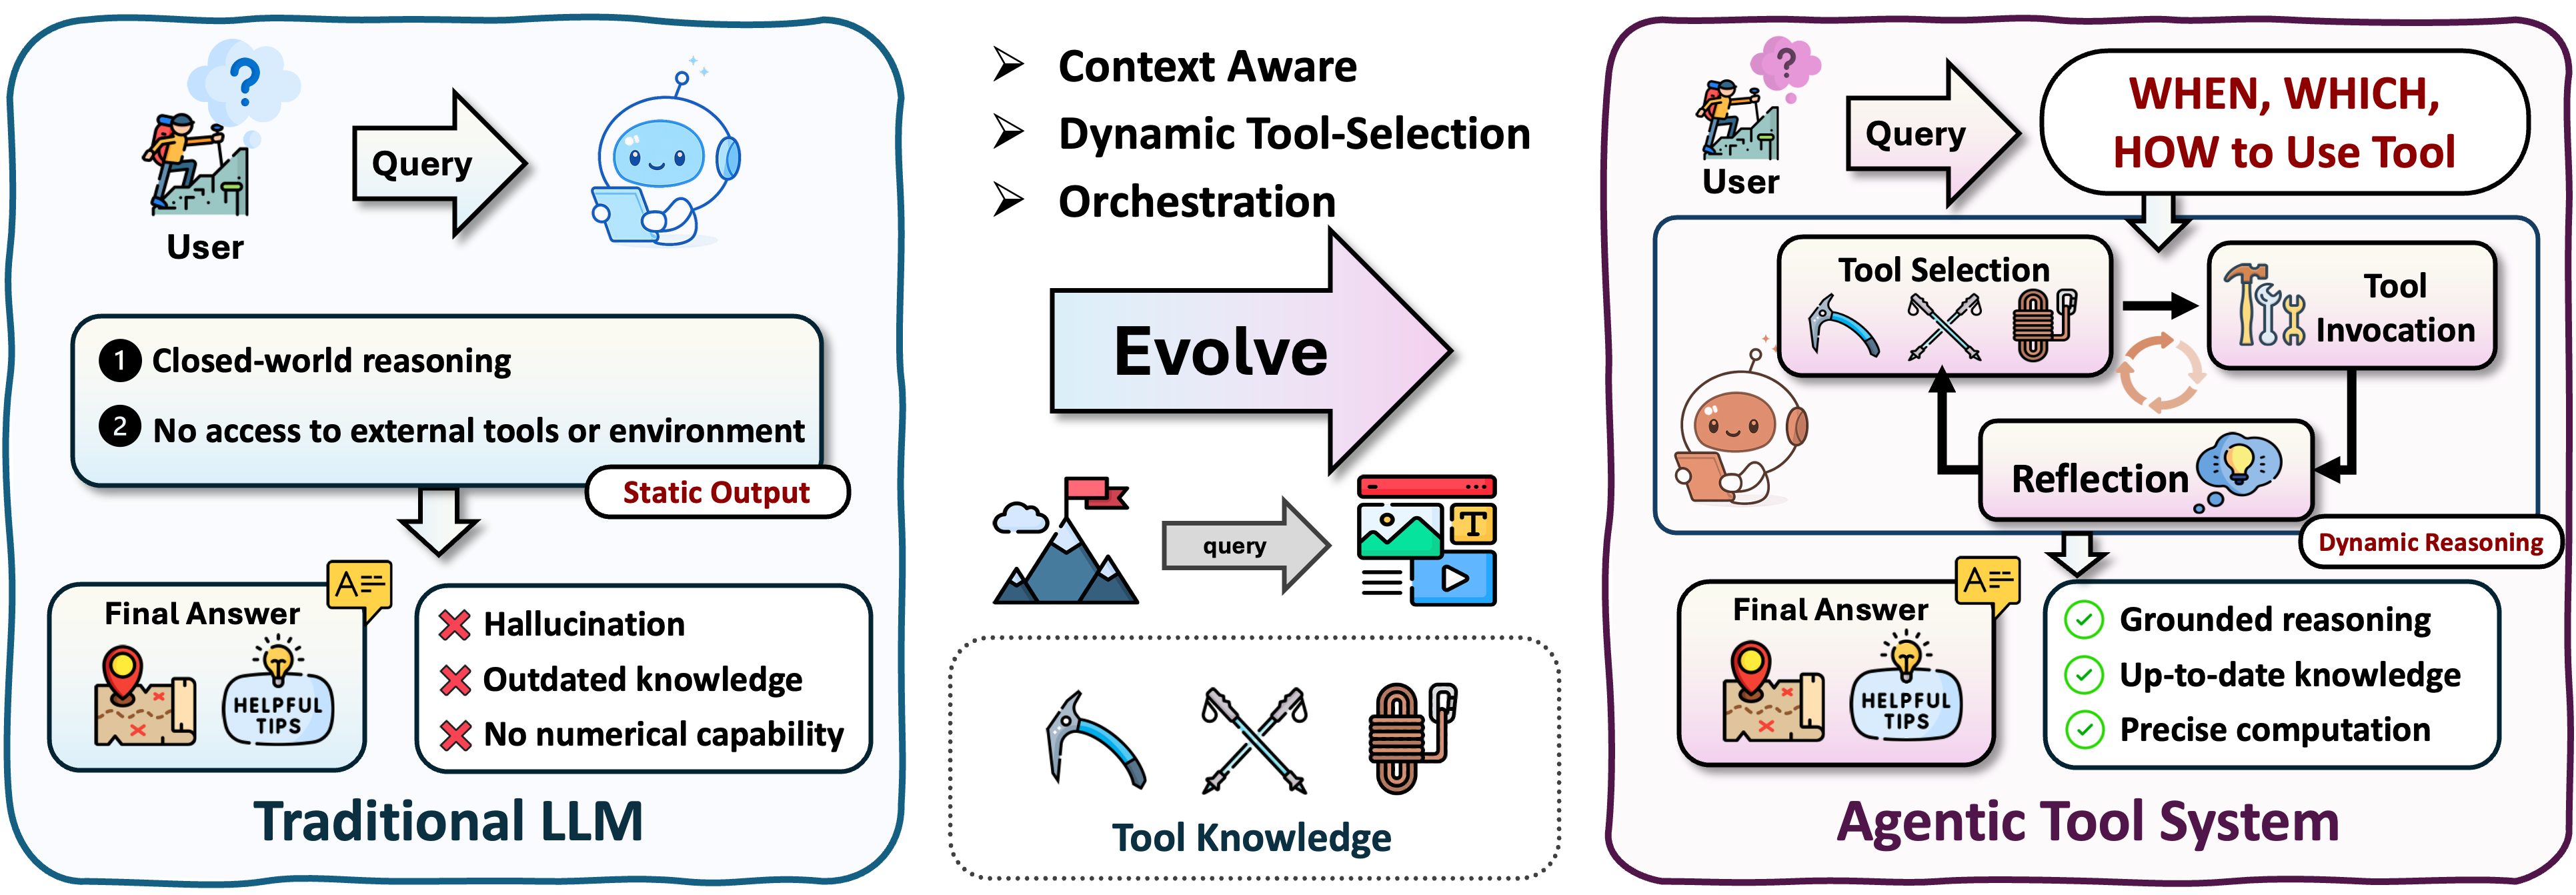
\includegraphics[width=\linewidth]{arxiv/figs/tool_use.png}
    \caption{Comparison between \textbf{traditional LLM} and \textbf{agentic tool-use} systems. While traditional models operate in a closed world with fixed reasoning, agentic tool-use systems enable dynamic selection, orchestration, and integration of external tools, allowing agents to extend reasoning, improve precision, and dynamically adapt across domains.}
    \label{fig:tool_use}
\end{figure}



\subsubsection{Post-training Tool-integration} Tool integration \citep{yao2023react, qu2025tool,shi2025tool} with post-training techniques has emerged as a key strategy for addressing the inherent limitations of LLMs or LRMs, such as outdated knowledge, limited computational precision, and shallow multi-step reasoning. By \textit{learning how to interact with external tools}, reasoning models can dynamically access up-to-date information, execute precise symbolic or numerical computations, and decompose complex tasks into grounded, tool-assisted reasoning steps \citep{wang2024empowering,yang2024buffer,singh2025agentic, cheng2024seeclick, zou2025reasonflux}. With tools as intermediaries, models are enriched and augmented by external capabilities, enabling the generation of more accurate and generalizable agentic reasoning trajectories \citep{nam2024using,yuan2024easytool,wu2025agentic}.

\paragraph{Bootstrapping of Tool Use via SFT.} \space Early works on tool-integration \citep{yao2023react, schick2023toolformer, DBLP:conf/iclr/QinLYZYLLCTQZHT24, DBLP:journals/corr/abs-2306-05301, lu2023chameleon, song2023restgpt, prasad2023adapt, yin2023agent, shi2024learning} primarily apply supervised fine-tuning (SFT) over curated tool-use reasoning steps, where models were trained to imitate demonstrations of search queries, code executions, or API calls. The SFT stage provided an initial competency in invoking tools, interpreting tool outputs, and integrating the results into coherent reasoning chains \citep{song2023restgpt, shinn2023reflexion}. For example, 
Toolformer \cite{schick2023toolformer} introduces a self-supervised framework in which large language models generate, validate, and retain useful API calls within unlabeled text, followed by fine-tuning on the filtered data to enhance factual accuracy and practical utility. 
ToolLLM \cite{DBLP:conf/iclr/QinLYZYLLCTQZHT24} further scales SFT training to over 16,000 real-world APIs, applying supervised fine-tuning on massive curated demonstrations to endow models with robust planning and invocation abilities. ToolAlpaca \cite{DBLP:journals/corr/abs-2306-05301} extends the idea to compact LLMs by automatically constructing a diverse toolset and generating multi-turn tool-use dialogues via multi-agent simulation, followed by fine-tuning to enable generalized tool-use even for previously unseen tools. While effective at bootstrapping tool-awareness, applying SFT along suffers from overfitting to the specific patterns in the training data \cite{kirk2023understanding, li2024preserving, o2024attributing, zou2025transformer}, leading to brittle tool-selection strategies and limited adaptability in unseen downstream application scenarios \citep{zeng2025itool,qian2025toolrl,yu2025demystifying}.

\paragraph{Mastery of Tool Use via RL.} \space Recent studies \citep{zhou2025sweet, qian2025toolrl, wei2025swe, chen2025learning, zhang2025rlvmr, jin2025search, zou2025autotool, dong2025reinforcement} leverages reinforcement learning (RL) during model post-training to go beyond imitation and achieve mastery in tool-integrated reasoning. With the integration of RL, models refine their tool-use strategies through outcome-driven rewards, learning \textit{when}, \textit{how}, and \textit{which} tools to invoke via trial and error \cite{chen2025learning, feng2025retool, dong2025reinforcement, sun2025zerosearch}. For instance, SWE-RL \citep{wei2025swe} optimizes code-editing policies on large-scale software evolution data, improving not only software issue resolution but also general reasoning skills. ReSearch \cite{chen2025learning} embeds search operations into multi-hop reasoning chains, enabling adaptive retrieval during complex QA. ReTool integrates real-time code execution into reasoning rollouts, leading to optimal performance on advanced math reasoning benchmarks. ToolRL \cite{qian2025toolrl} generalizes this paradigm to diverse toolsets by introducing principled reward designs for stable and scalable multi-tool learning. Across these settings, RL has been shown to yield more robust, adaptive, and generalizable tool-use policies than SFT alone, often transferring effectively to out-of-domain tasks \cite{team2025kimi1.5, comanici2025gemini, team2025kimi2, zeng2025glm, zou2025tattoo}.



\subsubsection{Orchestration-based Tool-integration} In real-world applications, tool use within complex systems often extends beyond the single-model, single-tool setting, requiring orchestration among multiple tools to complete complex tasks. This orchestration typically involves planning, sequencing, and managing dependencies across tools, i.e., ensuring that intermediate outputs are passed and transformed appropriately. Several early works \citep{shen2023hugginggpt, DBLP:journals/corr/abs-2303-16434, DBLP:conf/nips/HaoLWH23} explore this direction by devising strategies for the coordinated use of multiple tools, enabling systems to solve multi-stage tasks that no single tool can handle in isolation. Specifically, HuggingGPT \citep{shen2023hugginggpt} employs a centralized agent that leverages a language interface to plan which tools to invoke and when, enabling the solution of complex tasks requiring multiple tools in sequence. TaskMatrix.AI \citep{DBLP:journals/corr/abs-2303-16434} connects foundation models with millions of APIs, using the models to generate task-solution outlines and automatically matching certain sub-tasks to off-the-shelf models and systems with specialized functionalities. ToolkenGPT \citep{lu2025octotoolsagenticframeworkextensible} augments frozen language models with massive tool sets by encoding each tool as a special token during next-token prediction.

\paragraph{Agentic Pipelines for Tool Orchestration.} There are many frameworks designed to enable LLMs to call and orchestrate tools effectively. Most of the current agentic paradigm follows a “plan before action” strategy, where the model first generates a structured plan for tool use and then executes it. ToolPlanner \citep{liu2025toolplanner} introduces a two-stage reinforcement learning framework with path planning and feedback, supported by MGToolBench, to bridge the gap between API-heavy training data and real-world user instructions.
Tool-MVR \citep{DBLP:journals/corr/abs-2506-04625} enhances reliability and reflection through meta-verification of tool calls and exploration-based reflection learning, achieving strong gains over GPT-4 and other baselines.
More recently, 
OctoTools \citep{lu2025octotoolsagenticframeworkextensible} provides a training-free, extensible framework with standardized tool cards, a hierarchical planner, and an executor, showing broad improvements across multi-domain reasoning tasks.
Chain-of-Tools \citep{DBLP:journals/corr/abs-2503-16779} leverages frozen LLMs’ semantic representations to dynamically compose unseen tools in chain-of-thought reasoning, enabling generalization to massive tool pools without fine-tuning.
PyVision \cite{DBLP:journals/corr/abs-2507-07998} introduces an interactive, multi-turn framework that enables MLLMs to dynamically generate, execute, and refine Python-based tools, moving beyond static toolsets in visual reasoning. ConAgents \cite{shi2024learning} makes an initial extension of tool use frameworks for interactive multi-agent settings.
We are also glad to see emerging applications of such agentic tool orchestration frameworks in the chemistry domain \citep{DBLP:journals/corr/abs-2505-02484}.

\paragraph{Tool Representations for Orchestration.} Beyond designing orchestration pipelines, another line of research focuses on optimizing the tools themselves to facilitate more accurate selection, composition, and coordination during orchestration. ToolExpNet \citep{DBLP:conf/acl/ZhangCZCDL25} models tools and their usage experiences as a network that encodes semantic similarity and dependency relations, allowing LLMs to distinguish between similar tools and account for interdependencies during selection. 
T2Agent \citep{DBLP:journals/corr/abs-2505-19768} addresses multimodal misinformation detection by representing tools with standardized templates and using Bayesian optimization to select a task-relevant subset. Coupled with Monte Carlo Tree Search over this reduced action space, T2Agent enables efficient multi-source verification.
ToolChain* \citep{DBLP:conf/iclr/ZhuangC0MBRS024} frames the entire tool action space as a decision tree and applies A* search with task-specific cost functions to guide navigation. This representation allows efficient pruning of high-cost branches and identification of optimal tool-use paths.
ToolRerank \citep{DBLP:conf/coling/ZhengLLLLW24} refines tool retrieval by introducing adaptive truncation for seen vs. unseen tools and hierarchy-aware reranking to balance concentration (for single-tool queries) and diversity (for multi-tool queries).


\subsection{Agentic Search}


Single-agent Agentic Retrieval-Augmented Generation (RAG) systems embed reasoning and control into a centralized agent that governs the entire retrieval-generation loop.
Unlike traditional RAG pipelines~\cite{lewis2020retrieval, huang2024survey, yang2024crag} that perform fixed, one-shot retrieval before generation, agentic RAG agents dynamically control \textit{when}, \textit{what}, and \textit{how} to retrieve based on real-time reasoning needs. This enables the model to adapt retrieval strategies mid-inference, refine its queries, and better integrate evidence from multiple sources. Based on how the agent selects, refines, and integrates retrieved content during reasoning, we categorize single-agent Agentic RAG systems into three distinct architectural styles: \textit{in-context}, \textit{post-training}, and \textit{structure-enhanced} agentic RAG.  

\begin{figure}
    \centering
    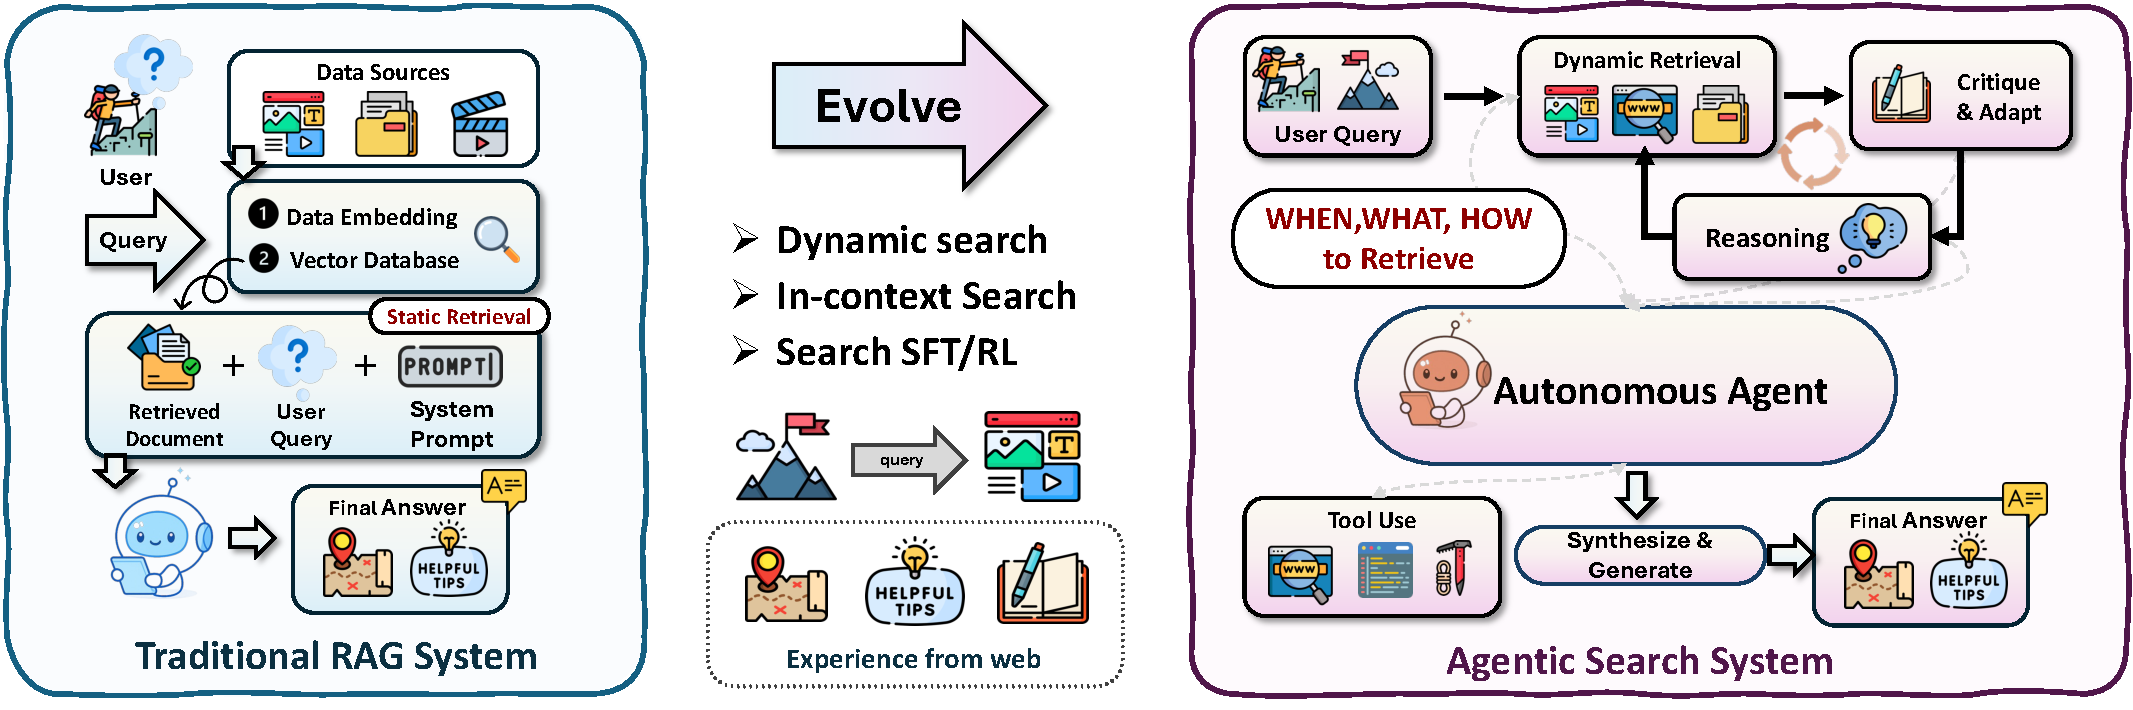
\includegraphics[width=\linewidth]{arxiv/figs/Agentic_search.pdf}
    \caption{Comparison between \textbf{traditional RAG} systems and \textbf{agentic search} systems. Traditional RAG relies on static retrieval over a vector database, while agentic search introduces autonomous decision-making for when, what, and how to retrieve, enabling dynamic search, in-context retrieval, critique-and-adapt loops, and tool use.}
    \label{fig:agentic_rag}
\end{figure}


\begin{table*}[!t]
\centering
\caption{
Representative \textbf{Agentic Search} systems categorized by \textit{Reasoning Structure}, \textit{Format}, and \textit{Tool Use}. 
{NL} denotes natural language traces used during reasoning, {Ops} refers to symbolic or graph operations, and {KG} stands for knowledge graph. 
Tool use includes search APIs, browser actions, or KG-based retrieval.
}
\renewcommand{\arraystretch}{1.15}
\setlength{\tabcolsep}{6pt}
\begin{tabular}{p{3cm}>{\centering\arraybackslash}p{3cm}>{\centering\arraybackslash}p{4cm}>{\centering\arraybackslash}p{5.5cm}}
\toprule
\textbf{Method} & \textbf{Structure} & \textbf{Format} & \textbf{Tool} \\
\midrule
\rowcolor[HTML]{F5F5F5}
\multicolumn{4}{l}{\textbf{Modality I: In-Context Agentic Search}} \\
ReAct~\cite{yao2023react} & Interleaved & NL + Actions & Search API \\
Self-Ask~\cite{press2022measuring} & Decomposed & NL Queries & Search API \\
IRCoT~\cite{trivedi2022interleaving} & Sequential & NL + CoT & Search API \\
Self-RAG~\cite{asai2023self} & Reflective & NL Self-check & Conditional Search \\
DeepRAG~\cite{guan2025deeprag} & Iterative & NL Feedback & Search API \\
\midrule
\rowcolor[HTML]{F5F5F5}
\multicolumn{4}{l}{\textbf{Modality II: Post-Training Agentic Search}} \\
Toolformer~\cite{schick2023toolformer} & Sequential & Tool Tokens & APIs, Search \\
INTERS~\cite{zhu2024inters} & Sequential & Instructions & Search API \\
WebGPT~\cite{nakano2021webgpt} & Sequential & NL + Browser & Web Search \\
RAG-RL~\cite{huang2025rag} & Decision & NL Policy & Evidence API \\
Search\text{-}R1~\cite{jin2025search} & Iterative & NL + Tokens & Live Web \\
Deep-Researcher~\cite{zheng2025deepresearcher} & Multi-step & NL Trajectories & Browser Tools \\
ReSearch~\cite{chen2025learning} & Step-wise & NL Steps & Search + Verifier \\
ReARTeR~\cite{sun2025rearter} & Reflective & NL Policy & Tool Cluster \\
\midrule
\rowcolor[HTML]{F5F5F5}
\multicolumn{4}{l}{\textbf{Modality III: Structure-Enhanced Agentic Search}} \\
Agent\text{-}G~\cite{leeagent} & Modular & NL + Graph Ops & KG Query \\
MC-Search~\cite{ning2025mc} & Multi-step & NL & Multimodal Search \\
GeAR~\cite{shen2025gear} & Graph & Graph Ops & KG Expansion \\
ARG~\cite{zhang2025learning} & Reflective & NL + Symbols & KG Traversal \\
\bottomrule
\end{tabular}
\label{tab:agentic_search_methods}
\end{table*}



\subsubsection{In-Context Search}

\paragraph{Interleaving Reasoning and Search.}

In-context agentic RAG systems embed retrieval behavior directly into the inference process of language models through carefully designed prompting strategies. Rather than training the model to learn retrieval behavior, these methods guide it to alternate between reasoning and search within a single forward pass, typically via few-shot exemplars or special tokens. A representative example is ReAct~\cite{yao2023react}, which interleaves Chain-of-Thought reasoning with tool-use commands such as \texttt{<Search>} to dynamically invoke external APIs or knowledge sources. Extensions such as Self-Ask~\cite{press2022measuring} and IRCoT~\cite{trivedi2022interleaving} go beyond sequential reasoning by prompting the model to recursively decompose questions and retrieve sub-evidence accordingly. More recent methods~\cite{asai2023self, li2024benchmarking, guan2025deeprag, ning2025mc} introduce reflective retrieval, where the model explicitly assesses whether it needs additional information at each step, deciding to retrieve only when necessary. These approaches require no additional training, making them highly flexible and deployable, but often rely on prompt engineering and may struggle with stability across diverse domains.

\paragraph{Structure-Enhanced Search.}

Structure-enhanced agentic RAG systems enhance retrieval-augmented generation by enabling a single agent to reason over symbolic knowledge sources such as knowledge graphs through dynamic querying, tool invocation, and reflective self-monitoring. Unlike static KG retrievers or query executors, these agents decide when to access structured knowledge, how to formulate graph-based queries, and whether retrieved information suffices for continuing the reasoning trajectory. Agent-G~\cite{leeagent} introduces a modular agentic architecture that integrates unstructured document retrieval with structured graph reasoning, using feedback loops and specialized retriever modules to ensure accurate multi-hop responses. MC-Search~\cite{ning2025mc} introduces five canonical reasoning topologies to model multimodal search-enhanced reasoning process, and proposes a end-to-end agentic RAG and step-wise evaluation pipeline to evaluate model's planning and retrieval fidelity across heterogeneous sources. Similarly, GeAR~\cite{shen2025gear} incorporates graph expansion operations into an agentic controller to address challenges in complex multi-hop queries, enhancing coherence across structured and unstructured sources. Beyond retrieval orchestration, ARG~\cite{zhang2025learning} proposes a fully end-to-end agentic framework for reasoning over knowledge graphs via active self-reflection. The model autonomously determines when to retrieve, performs iterative critique based on symbolic inputs, and exhibits interpretable, step-wise reasoning behavior over graphs. Together, these systems represent a shift from passive graph access to active, feedback-driven symbolic reasoning, highlighting the potential of structured agentic RAG to achieve both factual reliability and interpretability.

\subsubsection{Post-Training Search}
Post-training agentic RAG methods endow language models with retrieval-aware capabilities by fine-tuning them to make informed decisions throughout multi-step reasoning. Unlike in-context prompting, these approaches train models, either via supervised fine-tuning (SFT) or reinforcement learning (RL), to determine when retrieval is necessary, how to formulate queries, and how to incorporate retrieved evidence.

\paragraph{SFT-Based Agentic Search.} These methods construct curated or synthetic datasets that interleave retrieval operations with natural language reasoning, and subsequently apply supervised fine-tuning to instill retrieval-aware capabilities into the model. Toolformer~\cite{schick2023toolformer} introduces a self-supervised approach to annotate tool-use behaviors within model-generated text, enabling LLMs to learn when and how to invoke tools such as web search or calculators. INTERS~\cite{zhu2024inters} extends this direction by performing instruction-based fine-tuning over a diverse, multi-task dataset compiled from over 40 sources, capturing a wide spectrum of retrieval-reasoning patterns. This class of methods benefits from scalable data generation pipelines~\cite{mao2024rag, zhang2024raft, li2025search}, which minimize the need for human annotation. Instructional reformulation techniques~\cite{lin2023ra,zhu2024inters, nguyen2024sfr} further enhance generalization by aligning tasks with human-preferred formats and reasoning.

\paragraph{RL-Based Agentic Search.} These methods optimize retrieval-aware behaviors through reward signals that reflect answer quality, factuality, or user preferences. WebGPT~\cite{nakano2021webgpt} introduces reward modeling to supervise search-augmented chains aligned with human judgment, while RAG-RL~\cite{huang2025rag} formulates retrieval as a sequential decision-making task over evidence access. More recent efforts such as Search-R1~\cite{jin2025search} and Deep-Researcher~\cite{zheng2025deepresearcher} go further by training agents to dynamically issue retrieval actions (e.g., generating \texttt{<Search>} tokens mid-reasoning) and operate in open-ended environments such as the live web. These agents exhibit emergent capabilities such as iterative decomposition, re-verification, and evidence planning. Finally, systems like ReSearch~\cite{chen2025learning} and ReARTeR~\cite{sun2025rearter} pursue not only accurate answers but also interpretable and faithful reasoning trajectories, highlighting the potential of reinforcement-learned retrievers to act as controllable and reflective agents.



